\documentclass{article}
\usepackage{pgfplots}
\pgfplotsset{compat=1.18}
\begin{document}

\begin{figure}[htbp]
\centering
\begin{tikzpicture}
\begin{axis}[
    width=0.8\textwidth,
    height=0.6\textwidth,
    xlabel={log2(SIZE)},
    ylabel={L1 Miss Rate},
    title={L1 Miss Rate vs Cache Size},
    legend pos=north east,
    legend style={font=\tiny},
    grid=major
]
\addplot coordinates {(11.0,0.1477) (12.0,0.1002) (13.0,0.067) (14.0,0.0461) (15.0,0.0377) (16.0,0.0329) (17.0,0.0323) (18.0,0.0258) (19.0,0.0258) (20.0,0.0258)};
\addlegendentry{1}
\addplot coordinates {(11.0,0.1071) (12.0,0.0753) (13.0,0.0473) (14.0,0.0338) (15.0,0.0288) (16.0,0.0271) (17.0,0.0259) (18.0,0.0258) (19.0,0.0258) (20.0,0.0258)};
\addlegendentry{2}
\addplot coordinates {(11.0,0.0962) (12.0,0.0599) (13.0,0.0425) (14.0,0.0283) (15.0,0.0264) (16.0,0.026) (17.0,0.0258) (18.0,0.0258) (19.0,0.0258) (20.0,0.0258)};
\addlegendentry{4}
\addplot coordinates {(11.0,0.0907) (12.0,0.0537) (13.0,0.0395) (14.0,0.0277) (15.0,0.0262) (16.0,0.0259) (17.0,0.0258) (18.0,0.0258) (19.0,0.0258) (20.0,0.0258)};
\addlegendentry{8}
\addplot coordinates {(11.0,None) (12.0,None) (13.0,None) (14.0,None) (15.0,None) (16.0,None) (17.0,None) (18.0,None) (19.0,None) (20.0,None)};
\addlegendentry{-1}

\end{axis}
\end{tikzpicture}
\caption{L1 Miss Rate vs Cache Size}
\end{figure}

\begin{figure}[htbp]
\centering
\begin{tikzpicture}
\begin{axis}[
    width=0.8\textwidth,
    height=0.6\textwidth,
    xlabel={log2(SIZE)},
    ylabel={AAT},
    title={Average Access Time vs Cache Size},
    legend pos=north east,
    legend style={font=\tiny},
    grid=major
]
\addplot coordinates {(11.0,3.3955) (12.0,2.3674) (13.0,1.6576) (14.0,1.2246) (15.0,1.0744) (16.0,1.0232) (17.0,1.0765) (18.0,1.0113) (19.0,1.1233) (20.0,1.2559)};
\addlegendentry{1}
\addplot coordinates {(11.0,2.5391) (12.0,1.8457) (13.0,1.254) (14.0,0.9782) (15.0,0.909) (16.0,0.9088) (17.0,0.94) (18.0,1.0115) (19.0,1.1325) (20.0,1.2679)};
\addlegendentry{2}
\addplot coordinates {(11.0,None) (12.0,1.5252) (13.0,1.1509) (14.0,0.8663) (15.0,0.8624) (16.0,0.8921) (17.0,0.9468) (18.0,1.016) (19.0,1.1385) (20.0,1.262)};
\addlegendentry{4}
\addplot coordinates {(11.0,None) (12.0,None) (13.0,1.1124) (14.0,0.8621) (15.0,0.8659) (16.0,0.9034) (17.0,0.9665) (18.0,1.0214) (19.0,1.1447) (20.0,1.2703)};
\addlegendentry{8}
\addplot coordinates {(11.0,None) (12.0,None) (13.0,None) (14.0,None) (15.0,None) (16.0,None) (17.0,None) (18.0,None) (19.0,None) (20.0,None)};
\addlegendentry{-1}

\end{axis}
\end{tikzpicture}
\caption{Average Access Time vs Cache Size}
\end{figure}

\begin{figure}[htbp]
\centering
\begin{tikzpicture}
\begin{axis}[
    width=0.8\textwidth,
    height=0.6\textwidth,
    xlabel={log2(L1 SIZE)},
    ylabel={AAT},
    title={Average Access Time vs L1 Cache Size (with L2)},
    legend pos=north east,
    legend style={font=\tiny},
    grid=major
]
\addplot coordinates {(11.0,0.7802) (12.0,0.7771) (13.0,0.782) (14.0,0.7996) (15.0,0.8306) (16.0,0.8819) (17.0,0.948)};
\addlegendentry{1}
\addplot coordinates {(11.0,0.7986) (12.0,0.7918) (13.0,0.8021) (14.0,0.8171) (15.0,0.8562) (16.0,0.8923) (17.0,0.95)};
\addlegendentry{2}
\addplot coordinates {(11.0,None) (12.0,0.8021) (13.0,0.8039) (14.0,0.8242) (15.0,0.8616) (16.0,0.901) (17.0,0.9585)};
\addlegendentry{4}
\addplot coordinates {(11.0,None) (12.0,None) (13.0,0.8285) (14.0,0.8324) (15.0,0.8683) (16.0,0.9136) (17.0,0.9782)};
\addlegendentry{8}
\addplot coordinates {(11.0,None) (12.0,None) (13.0,None) (14.0,None) (15.0,None) (16.0,None) (17.0,None)};
\addlegendentry{-1}

\end{axis}
\end{tikzpicture}
\caption{Average Access Time vs L1 Cache Size (with L2)}
\end{figure}

\begin{figure}[htbp]
\centering
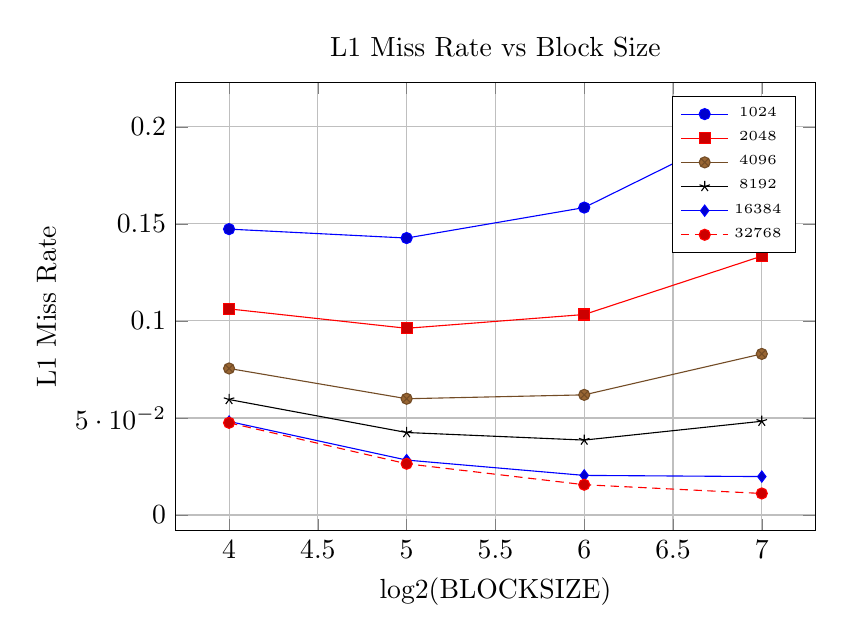
\begin{tikzpicture}
\begin{axis}[
    width=0.8\textwidth,
    height=0.6\textwidth,
    xlabel={log2(BLOCKSIZE)},
    ylabel={L1 Miss Rate},
    title={L1 Miss Rate vs Block Size},
    legend pos=north east,
    legend style={font=\tiny},
    grid=major
]
\addplot coordinates {(4.0,0.1473) (5.0,0.1427) (6.0,0.1584) (7.0,0.2036)};
\addlegendentry{1024}
\addplot coordinates {(4.0,0.1062) (5.0,0.0962) (6.0,0.1033) (7.0,0.1334)};
\addlegendentry{2048}
\addplot coordinates {(4.0,0.0755) (5.0,0.0599) (6.0,0.0619) (7.0,0.083)};
\addlegendentry{4096}
\addplot coordinates {(4.0,0.0595) (5.0,0.0425) (6.0,0.0386) (7.0,0.0483)};
\addlegendentry{8192}
\addplot coordinates {(4.0,0.0482) (5.0,0.0283) (6.0,0.0204) (7.0,0.0198)};
\addlegendentry{16384}
\addplot coordinates {(4.0,0.0475) (5.0,0.0264) (6.0,0.0156) (7.0,0.0111)};
\addlegendentry{32768}

\end{axis}
\end{tikzpicture}
\caption{L1 Miss Rate vs Block Size}
\end{figure}

\begin{figure}[htbp]
\centering
\begin{tikzpicture}
\begin{axis}[
    width=0.8\textwidth,
    height=0.6\textwidth,
    xlabel={log2(L1 SIZE)},
    ylabel={log2(L2 SIZE)},
    title={AAT vs L1 and L2 Cache Sizes},
    legend pos=north east,
    legend style={font=\tiny},
    grid=major
]
\addplot3[surf] coordinates {(10.0,15.0,None) (10.0,16.0,None) (10.0,17.0,None) (10.0,18.0,None) (10.0,19.0,None) (10.0,20.0,None) (11.0,15.0,None) (11.0,16.0,None) (11.0,17.0,None) (11.0,18.0,None) (11.0,19.0,None) (11.0,20.0,None) (12.0,15.0,0.8017) (12.0,16.0,0.7972) (12.0,17.0,0.7988) (12.0,18.0,0.8021) (12.0,19.0,0.8095) (12.0,20.0,0.817) (13.0,15.0,0.8063) (13.0,16.0,0.8012) (13.0,17.0,0.8015) (13.0,18.0,0.8039) (13.0,19.0,0.8091) (13.0,20.0,0.8144) (14.0,15.0,0.8287) (14.0,16.0,0.8239) (14.0,17.0,0.8226) (14.0,18.0,0.8242) (14.0,19.0,0.8277) (14.0,20.0,0.8312) (15.0,16.0,0.8619) (15.0,17.0,0.8601) (15.0,18.0,0.8616) (15.0,19.0,0.8648) (15.0,20.0,0.8681) (16.0,17.0,0.8996) (16.0,18.0,0.901) (16.0,19.0,0.9042) (16.0,20.0,0.9075)};

\end{axis}
\end{tikzpicture}
\caption{AAT vs L1 and L2 Cache Sizes}
\end{figure}

\begin{figure}[htbp]
\centering
\begin{tikzpicture}
\begin{axis}[
    width=0.8\textwidth,
    height=0.6\textwidth,
    xlabel={log2(L1 SIZE)},
    ylabel={log2(L2 SIZE)},
    title={EDP vs L1 and L2 Cache Sizes},
    legend pos=north east,
    legend style={font=\tiny},
    grid=major
]
\addplot3[surf] coordinates {(10.0,15.0,None) (10.0,16.0,None) (10.0,17.0,None) (10.0,18.0,None) (10.0,19.0,None) (10.0,20.0,None) (11.0,15.0,None) (11.0,16.0,None) (11.0,17.0,None) (11.0,18.0,None) (11.0,19.0,None) (11.0,20.0,None) (12.0,15.0,73885413.4163) (12.0,16.0,72915713.4677) (12.0,17.0,77664335.8234) (12.0,18.0,84466483.6989) (12.0,19.0,98574319.5847) (12.0,20.0,121910883.1549) (13.0,15.0,70402761.597) (13.0,16.0,68614171.7189) (13.0,17.0,72008604.2251) (13.0,18.0,77288670.6886) (13.0,19.0,88194735.6986) (13.0,20.0,106225902.4862) (14.0,15.0,82350455.2578) (14.0,16.0,79807701.1641) (14.0,17.0,82104775.9378) (14.0,18.0,86273935.1903) (14.0,19.0,94851120.7937) (14.0,20.0,109001894.8549) (15.0,16.0,106821784.7127) (15.0,17.0,108746003.4077) (15.0,18.0,112698872.2312) (15.0,19.0,120825027.9592) (15.0,20.0,134169789.4768) (16.0,17.0,144658580.5199) (16.0,18.0,148298915.0474) (16.0,19.0,155792289.3387) (16.0,20.0,168005515.2908)};

\end{axis}
\end{tikzpicture}
\caption{EDP vs L1 and L2 Cache Sizes}
\end{figure}

\begin{figure}[htbp]
\centering
\begin{tikzpicture}
\begin{axis}[
    width=0.8\textwidth,
    height=0.6\textwidth,
    xlabel={log2(L1 SIZE)},
    ylabel={AAT},
    title={AAT vs L1 Cache Size (with Victim Cache)},
    legend pos=north east,
    legend style={font=\tiny},
    grid=major
]
\addplot coordinates {(10.0,0.7861) (11.0,0.7802) (12.0,0.7771) (13.0,0.782) (14.0,0.7996) (15.0,0.8306)};
\addlegendentry{(1, 0)}
\addplot coordinates {(10.0,0.7905) (11.0,0.7839) (12.0,0.7824) (13.0,0.7857) (14.0,0.8022) (15.0,0.832)};
\addlegendentry{(1, 4)}
\addplot coordinates {(10.0,0.7845) (11.0,0.78) (12.0,0.7799) (13.0,0.7838) (14.0,0.8014) (15.0,0.8317)};
\addlegendentry{(1, 8)}
\addplot coordinates {(10.0,0.7769) (11.0,0.7751) (12.0,0.7752) (13.0,0.7811) (14.0,0.8007) (15.0,0.8313)};
\addlegendentry{(1, 16)}
\addplot coordinates {(10.0,None) (11.0,0.7986) (12.0,0.7918) (13.0,0.8021) (14.0,0.8171) (15.0,0.8562)};
\addlegendentry{(2, 0)}
\addplot coordinates {(10.0,None) (11.0,None) (12.0,0.8021) (13.0,0.8039) (14.0,0.8242) (15.0,0.8616)};
\addlegendentry{(4, 0)}

\end{axis}
\end{tikzpicture}
\caption{AAT vs L1 Cache Size (with Victim Cache)}
\end{figure}
\end{document}